\documentclass[12pt,a4paper,]{report}
\usepackage{lmodern}

% Overwrite \begin{figure}[htbp] with \begin{figure}[H]
\usepackage{float}
\let\origfigure=\figure
\let\endorigfigure=\endfigure
\renewenvironment{figure}[1][]{%
\origfigure[b]
}{%
\endorigfigure
}

% fix for pandoc 1.14
\providecommand{\tightlist}{%
  \setlength{\itemsep}{0pt}\setlength{\parskip}{0pt}}

% TP: hack to truncate list of figures/tables.
\usepackage{truncate}
\usepackage{caption}
\usepackage{tocloft}
% TP: end hack

\usepackage{amssymb,amsmath}
\usepackage{ifxetex,ifluatex}

% Only use fixltx2e if using pre-2015 kernels
\begingroup\expandafter\expandafter\expandafter\endgroup
\expandafter\ifx\csname IncludeInRelease\endcsname\relax
  \usepackage{fixltx2e}
\fi

\ifnum 0\ifxetex 1\fi\ifluatex 1\fi=0 % if pdftex
  \usepackage[T1]{fontenc}
  \usepackage[utf8]{inputenc}
\else % if luatex or xelatex
  \ifxetex
    \usepackage{mathspec}
    \usepackage{xltxtra,xunicode}
  \else
    \usepackage{fontspec}
  \fi
  \defaultfontfeatures{Mapping=tex-text,Scale=MatchLowercase}
  \newcommand{\euro}{€}
\fi
% use upquote if available, for straight quotes in verbatim environments
\IfFileExists{upquote.sty}{\usepackage{upquote}}{}
% use microtype if available
\IfFileExists{microtype.sty}{%
\usepackage{microtype}
\UseMicrotypeSet[protrusion]{basicmath} % disable protrusion for tt fonts
}{}
\usepackage{color}
\usepackage{fancyvrb}
\newcommand{\VerbBar}{|}
\newcommand{\VERB}{\Verb[commandchars=\\\{\}]}
\DefineVerbatimEnvironment{Highlighting}{Verbatim}{commandchars=\\\{\}}
% Add ',fontsize=\small' for more characters per line
\newenvironment{Shaded}{}{}
\newcommand{\AlertTok}[1]{\textcolor[rgb]{1.00,0.00,0.00}{\textbf{#1}}}
\newcommand{\AnnotationTok}[1]{\textcolor[rgb]{0.38,0.63,0.69}{\textbf{\textit{#1}}}}
\newcommand{\AttributeTok}[1]{\textcolor[rgb]{0.49,0.56,0.16}{#1}}
\newcommand{\BaseNTok}[1]{\textcolor[rgb]{0.25,0.63,0.44}{#1}}
\newcommand{\BuiltInTok}[1]{#1}
\newcommand{\CharTok}[1]{\textcolor[rgb]{0.25,0.44,0.63}{#1}}
\newcommand{\CommentTok}[1]{\textcolor[rgb]{0.38,0.63,0.69}{\textit{#1}}}
\newcommand{\CommentVarTok}[1]{\textcolor[rgb]{0.38,0.63,0.69}{\textbf{\textit{#1}}}}
\newcommand{\ConstantTok}[1]{\textcolor[rgb]{0.53,0.00,0.00}{#1}}
\newcommand{\ControlFlowTok}[1]{\textcolor[rgb]{0.00,0.44,0.13}{\textbf{#1}}}
\newcommand{\DataTypeTok}[1]{\textcolor[rgb]{0.56,0.13,0.00}{#1}}
\newcommand{\DecValTok}[1]{\textcolor[rgb]{0.25,0.63,0.44}{#1}}
\newcommand{\DocumentationTok}[1]{\textcolor[rgb]{0.73,0.13,0.13}{\textit{#1}}}
\newcommand{\ErrorTok}[1]{\textcolor[rgb]{1.00,0.00,0.00}{\textbf{#1}}}
\newcommand{\ExtensionTok}[1]{#1}
\newcommand{\FloatTok}[1]{\textcolor[rgb]{0.25,0.63,0.44}{#1}}
\newcommand{\FunctionTok}[1]{\textcolor[rgb]{0.02,0.16,0.49}{#1}}
\newcommand{\ImportTok}[1]{#1}
\newcommand{\InformationTok}[1]{\textcolor[rgb]{0.38,0.63,0.69}{\textbf{\textit{#1}}}}
\newcommand{\KeywordTok}[1]{\textcolor[rgb]{0.00,0.44,0.13}{\textbf{#1}}}
\newcommand{\NormalTok}[1]{#1}
\newcommand{\OperatorTok}[1]{\textcolor[rgb]{0.40,0.40,0.40}{#1}}
\newcommand{\OtherTok}[1]{\textcolor[rgb]{0.00,0.44,0.13}{#1}}
\newcommand{\PreprocessorTok}[1]{\textcolor[rgb]{0.74,0.48,0.00}{#1}}
\newcommand{\RegionMarkerTok}[1]{#1}
\newcommand{\SpecialCharTok}[1]{\textcolor[rgb]{0.25,0.44,0.63}{#1}}
\newcommand{\SpecialStringTok}[1]{\textcolor[rgb]{0.73,0.40,0.53}{#1}}
\newcommand{\StringTok}[1]{\textcolor[rgb]{0.25,0.44,0.63}{#1}}
\newcommand{\VariableTok}[1]{\textcolor[rgb]{0.10,0.09,0.49}{#1}}
\newcommand{\VerbatimStringTok}[1]{\textcolor[rgb]{0.25,0.44,0.63}{#1}}
\newcommand{\WarningTok}[1]{\textcolor[rgb]{0.38,0.63,0.69}{\textbf{\textit{#1}}}}
\usepackage{longtable,booktabs}
\usepackage{graphicx}
\makeatletter
\def\maxwidth{\ifdim\Gin@nat@width>\linewidth\linewidth\else\Gin@nat@width\fi}
\def\maxheight{\ifdim\Gin@nat@height>\textheight\textheight\else\Gin@nat@height\fi}
\makeatother
% Scale images if necessary, so that they will not overflow the page
% margins by default, and it is still possible to overwrite the defaults
% using explicit options in \includegraphics[width, height, ...]{}
\setkeys{Gin}{width=\maxwidth,height=\maxheight,keepaspectratio}
\ifxetex
  \usepackage[setpagesize=false, % page size defined by xetex
              unicode=false, % unicode breaks when used with xetex
              xetex]{hyperref}
\else
  \usepackage[unicode=true]{hyperref}
\fi
\hypersetup{breaklinks=true,
            bookmarks=true,
            pdfauthor={Firstname Surname},
            pdftitle={This is the title of the thesis},
            colorlinks=true,
            citecolor=blue,
            urlcolor=blue,
            linkcolor=magenta,
            pdfborder={0 0 0}}
\urlstyle{same}  % don't use monospace font for urls
\setlength{\parindent}{0pt}
\setlength{\parskip}{6pt plus 2pt minus 1pt}
\setlength{\emergencystretch}{3em}  % prevent overfull lines
\setcounter{secnumdepth}{5}

% % \newlength{\cslhangindent}
% \setlength{\cslhangindent}{1.5em}
% \newenvironment{cslreferences}%
%   {}%
%   {\par}
% 
\newlength{\cslhangindent}
\setlength{\cslhangindent}{1.5em}
\newlength{\csllabelwidth}
\setlength{\csllabelwidth}{3em}
\newenvironment{CSLReferences}[2] % #1 hanging-ident, #2 entry spacing
 {% don't indent paragraphs
  \setlength{\parindent}{0pt}
  % turn on hanging indent if param 1 is 1
  \ifodd #1 \everypar{\setlength{\hangindent}{\cslhangindent}}\ignorespaces\fi
  % set entry spacing
  \ifnum #2 > 0
  \setlength{\parskip}{#2\baselineskip}
  \fi
 }%
 {}
\usepackage{calc}
\newcommand{\CSLBlock}[1]{#1\hfill\break}
\newcommand{\CSLLeftMargin}[1]{\parbox[t]{\csllabelwidth}{#1}}
\newcommand{\CSLRightInline}[1]{\parbox[t]{\linewidth - \csllabelwidth}{#1}\break}
\newcommand{\CSLIndent}[1]{\hspace{\cslhangindent}#1}



% Table of contents formatting
\renewcommand{\contentsname}{Table of Contents}
\setcounter{tocdepth}{3}

% Headers and page numbering
\usepackage{fancyhdr}
\pagestyle{plain}

% Following package is used to add background image to front page
\usepackage{wallpaper}

% Table package
\usepackage{ctable}% http://ctan.org/pkg/ctable

% Deal with 'LaTeX Error: Too many unprocessed floats.'
\usepackage{morefloats}
% or use \extrafloats{100}
% add some \clearpage

% % Chapter header
% \usepackage{titlesec, blindtext, color}
% \definecolor{gray75}{gray}{0.75}
% \newcommand{\hsp}{\hspace{20pt}}
% \titleformat{\chapter}[hang]{\Huge\bfseries}{\thechapter\hsp\textcolor{gray75}{|}\hsp}{0pt}{\Huge\bfseries}

% % Fonts and typesetting
% \setmainfont[Scale=1.1]{Helvetica}
% \setsansfont[Scale=1.1]{Verdana}

% FONTS
\usepackage{xunicode}
\usepackage{xltxtra}
\defaultfontfeatures{Mapping=tex-text} % converts LaTeX specials (``quotes'' --- dashes etc.) to unicode
% \setromanfont[Scale=1.01,Ligatures={Common},Numbers={OldStyle}]{Palatino}
% \setromanfont[Scale=1.01,Ligatures={Common},Numbers={OldStyle}]{Adobe Caslon Pro}
%Following line controls size of code chunks
% \setmonofont[Scale=0.9]{Monaco}
%Following line controls size of figure legends
% \setsansfont[Scale=1.2]{Optima Regular}

% CODE BLOCKS
\usepackage[utf8]{inputenc}
\usepackage{listings}
\usepackage{color}

% JAVA CODE BLOCKS
%\definecolor{backcolour}{RGB}{242,242,242}
%\definecolor{javared}{rgb}{0.6,0,0}
%\definecolor{javagreen}{rgb}{0.25,0.5,0.35}
%\definecolor{javapurple}{rgb}{0.5,0,0.35}
%\definecolor{javadocblue}{rgb}{0.25,0.35,0.75}

\lstdefinestyle{javaCodeStyle}{
  language=Java,                         % the language of the code
  backgroundcolor=\color{backcolour},    % choose the background color; you must add \usepackage{color} or \usepackage{xcolor}
  basicstyle=\fontsize{10}{8}\sffamily,
  breakatwhitespace=false,
  breaklines=true,
  keywordstyle=\color{javapurple}\bfseries,
  stringstyle=\color{javared},
  commentstyle=\color{javagreen},
  morecomment=[s][\color{javadocblue}]{/**}{*/},
  captionpos=t,                          % sets the caption-position to bottom
  frame=single,                          % adds a frame around the code
  numbers=left,
  numbersep=10pt,                         % margin between number and code block
  keepspaces=true,                       % keeps spaces in text, useful for keeping indentation of code (possibly needs columns=flexible)
  columns=fullflexible,
  showspaces=false,                      % show spaces everywhere adding particular underscores; it overrides 'showstringspaces'
  showstringspaces=false,                % underline spaces within strings only
  showtabs=false,                        % show tabs within strings adding particular underscores
  tabsize=2                              % sets default tabsize to 2 spaces
}

%Attempt to set math size
%First size must match the text size in the document or command will not work
%\DeclareMathSizes{display size}{text size}{script size}{scriptscript size}.
%\DeclareMathSizes{12}{13}{7}{7}

% ---- CUSTOM AMPERSAND
% \newcommand{\amper}{{\fontspec[Scale=.95]{Adobe Caslon Pro}\selectfont\itshape\&}}

% HEADINGS
\usepackage{sectsty}
\usepackage[normalem]{ulem}
\sectionfont{\rmfamily\mdseries\Large}
\subsectionfont{\rmfamily\mdseries\scshape\large}
\subsubsectionfont{\rmfamily\bfseries\upshape\large}
% \sectionfont{\rmfamily\mdseries\Large}
% \subsectionfont{\rmfamily\mdseries\scshape\normalsize}
% \subsubsectionfont{\rmfamily\bfseries\upshape\normalsize}

% Set figure legends and captions to be smaller sized sans serif font
\usepackage[font={footnotesize,sf}]{caption}

\usepackage{siunitx}

% Adjust spacing between lines to 1.5
\usepackage{setspace}
% \onehalfspacing
\doublespacing
\raggedbottom

% Set margins
\usepackage[top=1.5in,bottom=1.5in,left=1.5in,right=1.4in]{geometry}
\setlength\parindent{0.5in} % indent at start of paragraphs (set to 0.3?)
\setlength{\parskip}{9pt}
\usepackage{indentfirst}

% Add space between pararaphs
% http://texblog.org/2012/11/07/correctly-typesetting-paragraphs-in-latex/
% \usepackage{parskip}
% \setlength{\parskip}{\baselineskip}

% Set colour of links to black so that they don't show up when printed
\usepackage{hyperref}
\hypersetup{colorlinks=false, linkcolor=black}

% Tables
\usepackage{booktabs}
\usepackage{threeparttable}
\usepackage{array}
\usepackage{makecell}
\newcolumntype{x}[1]{%
>{\centering\arraybackslash}m{#1}}%

% Allow for long captions and float captions on opposite page of figures
% \usepackage[rightFloats, CaptionBefore]{fltpage}

% Don't let floats cross subsections
% \usepackage[section,subsection]{extraplaceins}

% Rotate images and tables
\usepackage{float}
\usepackage{pdfpages}
\usepackage{pdflscape}
\usepackage{graphicx}
\usepackage{rotating}

% Custom math
\usepackage{bbold}
\DeclareMathOperator*{\argmin}{\arg\!\min}

\begin{document}


\begin{titlepage}
    \begin{center}

    % Delete the following line
    % to remove the UCL header logo
    \ThisULCornerWallPaper{1.0}{style/univ_logo.eps}

        \vspace*{2.5cm}

        \huge
        This is the title of the thesis

                \vspace{.5cm}

        \Large
        This is the subtitle of the thesis
        

        \vspace{1.5cm}

        \Large
        Firstname Surname

        \vspace{1.5cm}

        \normalsize
        A thesis presented for the degree of\\
        Doctor of Philosophy

        \vfill

        \normalsize
        Supervised by:\\
        Professor Louis Fage \\ Captain J. Y. Cousteau

        \vspace{0.8cm}

        % Uncomment the following line
        % to add a centered university logo
        % \includegraphics[width=0.4\textwidth]{style/univ_logo.eps}

        \normalsize
        University College London, UK\\
        January 2015

        % Except where otherwise noted, content in this thesis is licensed under a Creative Commons Attribution 4.0 License (http://creativecommons.org/licenses/by/4.0), which permits unrestricted use, distribution, and reproduction in any medium, provided the original work is properly cited. Copyright 2015,Tom Pollard.

    \end{center}
\end{titlepage}


% This is where the converted markdown files will go 
\vspace*{\fill}

\noindent \textit{
I, AUTHORNAME confirm that the work presented in this thesis is my own. Where information has been derived from other sources, I confirm that this has been indicated in the thesis.
} \vspace*{\fill} \pagenumbering{gobble} \newpage

\hypertarget{abstract}{%
\chapter*{Abstract}\label{abstract}}
\addcontentsline{toc}{chapter}{Abstract}

Lorem ipsum dolor sit amet, consectetur adipiscing elit. Nam et turpis
gravida, lacinia ante sit amet, sollicitudin erat. Aliquam efficitur
vehicula leo sed condimentum. Phasellus lobortis eros vitae rutrum
egestas. Vestibulum ante ipsum primis in faucibus orci luctus et
ultrices posuere cubilia Curae; Donec at urna imperdiet, vulputate orci
eu, sollicitudin leo. Donec nec dui sagittis, malesuada erat eget,
vulputate tellus. Nam ullamcorper efficitur iaculis. Mauris eu vehicula
nibh. In lectus turpis, tempor at felis a, egestas fermentum massa.

\pagenumbering{roman}
\setcounter{page}{1}

\hypertarget{acknowledgements}{%
\chapter*{Acknowledgements}\label{acknowledgements}}
\addcontentsline{toc}{chapter}{Acknowledgements}

Interdum et malesuada fames ac ante ipsum primis in faucibus. Aliquam
congue fermentum ante, semper porta nisl consectetur ut. Duis ornare sit
amet dui ac faucibus. Phasellus ullamcorper leo vitae arcu ultricies
cursus. Duis tristique lacus eget metus bibendum, at dapibus ante
malesuada. In dictum nulla nec porta varius. Fusce et elit eget sapien
fringilla maximus in sit amet dui.

Mauris eget blandit nisi, faucibus imperdiet odio. Suspendisse blandit
dolor sed tellus venenatis, venenatis fringilla turpis pretium. Donec
pharetra arcu vitae euismod tincidunt. Morbi ut turpis volutpat,
ultrices felis non, finibus justo. Proin convallis accumsan sem ac
vulputate. Sed rhoncus ipsum eu urna placerat, sed rhoncus erat
facilisis. Praesent vitae vestibulum dui. Proin interdum tellus ac velit
varius, sed finibus turpis placerat.

\newpage

\pagenumbering{gobble}

\tableofcontents

\newpage
\listoffigures

\newpage

\listoftables

\newpage

\hypertarget{abbreviations}{%
\chapter*{Abbreviations}\label{abbreviations}}
\addcontentsline{toc}{chapter}{Abbreviations}

\begin{tabbing}
\textbf{API}~~~~~~~~~~~~ \= \textbf{A}pplication \textbf{P}rogramming \textbf{I}nterface \\  
\textbf{JSON} \> \textbf{J}ava\textbf{S}cript \textbf{O}bject \textbf{N}otation \\  
\end{tabbing}

\newpage

\setcounter{page}{1}
\pagenumbering{arabic}
\doublespacing
\setlength{\parindent}{0.5in}

\hypertarget{introduction-with-a-citation}{%
\chapter{Introduction, with a
citation}\label{introduction-with-a-citation}}

\hypertarget{background}{%
\section{Background}\label{background}}

This is the introduction. Quisque finibus aliquet cursus. Integer in
pellentesque tellus. Duis eu dignissim nulla, a porttitor enim. Quisque
vehicula leo non ultrices finibus. Duis vehicula quis sem sit amet
sollicitudin. Integer neque est, pharetra et auctor vel, iaculis
interdum lectus.

To include a citation to the text, just add the citation key shown in
the references.bib file. The style of the citation is determined by the
ref\_format.csl file. For example, in The Living Sea you can find
pictures of the Calypso (Cousteau Jacques \& Dugan James 1963).

In neque mauris, maximus at sapien a, iaculis dignissim justo. Aliquam
erat volutpat. Praesent varius risus auctor est ultricies, sit amet
consequat nisi laoreet. Suspendisse non est et mauris pharetra sagittis
non porta justo. Praesent malesuada metus ut sapien sodales ornare.

\hypertarget{the-middle-bit}{%
\section{The middle bit}\label{the-middle-bit}}

This is the middle bit. Phasellus quis ex in ipsum pellentesque lobortis
tincidunt sed massa. Nullam euismod sem quis dictum condimentum.
Suspendisse risus metus, elementum eu congue quis, viverra ac metus.
Donec non lectus at lectus euismod laoreet pharetra semper dui. Donec
sed eleifend erat, vel ultrices nibh. Nam scelerisque turpis ac nunc
mollis, et rutrum nisl luctus.

Duis faucibus vestibulum elit, sit amet lobortis libero. Class aptent
taciti sociosqu ad litora torquent per conubia nostra, per inceptos
himenaeos. Sed at cursus nibh. Sed accumsan imperdiet interdum. Proin id
facilisis tortor. Proin posuere a neque nec iaculis. Suspendisse
potenti. Nullam hendrerit ante mi, vitae iaculis dui laoreet eu.

Cras eleifend velit diam, eu viverra mi volutpat ut. Cum sociis natoque
penatibus et magnis dis parturient montes, nascetur ridiculus mus. Donec
finibus leo nec dui imperdiet, tincidunt ornare orci venenatis. Maecenas
placerat efficitur est, eu blandit magna hendrerit eu.

\hypertarget{subsection-of-the-middle-bit}{%
\subsection{Subsection of the middle
bit}\label{subsection-of-the-middle-bit}}

This is a subsection of the middle bit. Quisque sit amet tempus arcu, ac
suscipit ante. Cras massa elit, pellentesque eget nisl ut, malesuada
rutrum risus. Nunc in venenatis mi. Curabitur sit amet suscipit eros,
non tincidunt nibh. Phasellus lorem lectus, iaculis non luctus eget,
tempus non risus. Suspendisse ut felis mi.

\hypertarget{summary-of-chapters}{%
\section{Summary of chapters}\label{summary-of-chapters}}

This is a brief outline of what went into each chapter, and a section
which shows how to reference headers (which are labelled automatically
for you).
\textbf{\protect\hyperlink{introduction-with-a-citation}{Chapter 1}}
shows how to use citations and how to reference section headers.
\textbf{\protect\hyperlink{literature-review-with-maths}{Chapter 2}}
shows how use and reference equations.
\textbf{\protect\hyperlink{first-research-study-with-code}{Chapter 3}}
shows how to use and reference code.
\textbf{\protect\hyperlink{research-containing-a-figure}{Chapter 4}}
shows how to use, reference, and resize pdf and jpg figures.
\textbf{\protect\hyperlink{research-containing-a-table}{Chapter 5}}
shows how to use and reference tables.
\textbf{\protect\hyperlink{final-research-study}{Chapter 6}} is truly
revolutionary (but shows nothing functional).
\textbf{\protect\hyperlink{appendix-1-some-extra-stuff}{Appendix 1}}
shows how to add chapters which are not numbered, as does
\textbf{\protect\hyperlink{appendix-2-some-more-extra-stuff}{Appendix
2}}. See the base
\href{https://github.com/tompollard/phd_thesis_markdown/blob/master/README.md}{\texttt{README.md}}
for how References are handled - leave \texttt{*\_references.md} alone,
and provide it to \texttt{pandoc} last.

Proin faucibus nibh sit amet augue blandit varius.

\hypertarget{literature-review-with-maths}{%
\chapter{Literature review, with
maths}\label{literature-review-with-maths}}

\hypertarget{introduction}{%
\section{Introduction}\label{introduction}}

This is the introduction. Duis in neque felis. In hac habitasse platea
dictumst. Cras eget rutrum elit. Pellentesque tristique venenatis
pellentesque. Cras eu dignissim quam, vel sodales felis. Vestibulum
efficitur justo a nibh cursus eleifend. Integer ultrices lorem at nunc
efficitur lobortis.

\hypertarget{the-middle}{%
\section{The middle}\label{the-middle}}

This is the literature review. Nullam quam odio, volutpat ac ornare
quis, vestibulum nec nulla. Aenean nec dapibus in
mL/min\textsuperscript{-1}. Mathematical formula can be inserted using
Latex and can be automatically numbered:

\begin{equation}f(x) = ax^3 + bx^2 + cx + d\label{eq:my_equation}\end{equation}

Nunc eleifend, ex a luctus porttitor, felis ex suscipit tellus, ut
sollicitudin sapien purus in libero. Nulla blandit eget urna vel tempus.
Praesent fringilla dui sapien, sit amet egestas leo sollicitudin at.

Later on in the text, you can reference Equation \ref{eq:my_equation}
and its mind-blowing ramifications. Pellentesque habitant morbi
tristique senectus et netus et malesuada fames ac turpis egestas. Sed
faucibus pulvinar volutpat. Ut semper fringilla erat non dapibus. Nunc
vitae felis eget purus placerat finibus laoreet ut nibh.

\hypertarget{a-complicated-math-equation}{%
\section{A complicated math
equation}\label{a-complicated-math-equation}}

The following raw text in markdown behind Equation
\ref{eq:my_complicated_equation} shows that you can fall back on
\LaTeX if it is more convenient for you. Note that this will only be
rendered in \texttt{thesis.pdf}

\begin{equation}
\begin{aligned}
    \hat{\theta}_g = \argmin_{\theta_g} \Big\{ - &\sum^{N}_{n=1}\Big( 1-\mathbb{1}[f(\pmb x^{(n)})]\Big)\log f\Big(\pmb x^{(n)} \\ 
    &+ g(\pmb x^{(n)};\theta_g)\Big) + \lambda|g(\pmb x^{(n)};\theta_g)|_2 \Big\} \ ,
\end{aligned}
\label{eq:my_complicated_equation}\end{equation}

\hypertarget{conclusion}{%
\section{Conclusion}\label{conclusion}}

This is the conclusion. Donec pulvinar molestie urna eu faucibus. In
tristique ut neque vel eleifend. Morbi ut massa vitae diam gravida
iaculis. Pellentesque habitant morbi tristique senectus et netus et
malesuada fames ac turpis egestas.

\begin{itemize}
\tightlist
\item
  first item in the list
\item
  second item in the list
\item
  third item in the list
\end{itemize}

\hypertarget{first-research-study-with-code}{%
\chapter{First research study, with
code}\label{first-research-study-with-code}}

\hypertarget{introduction-1}{%
\section{Introduction}\label{introduction-1}}

This is the introduction. Nam mollis congue tortor, sit amet convallis
tortor mollis eget. Fusce viverra ut magna eu sagittis. Vestibulum at
ultrices sapien, at elementum urna. Nam a blandit leo, non lobortis
quam. Aliquam feugiat turpis vitae tincidunt ultricies. Mauris
ullamcorper pellentesque nisl, vel molestie lorem viverra at.

\hypertarget{method}{%
\section{Method}\label{method}}

Suspendisse iaculis in lacus ut dignissim. Cras dignissim dictum
eleifend. Suspendisse potenti. Suspendisse et nisi suscipit, vestibulum
est at, maximus sapien. Sed ut diam tortor.

\hypertarget{subsection-1-with-example-code-block}{%
\subsection{Subsection 1 with example code
block}\label{subsection-1-with-example-code-block}}

This is the first part of the methodology. Cras porta dui a dolor
tincidunt placerat. Cras scelerisque sem et malesuada vestibulum.
Vivamus faucibus ligula ac sodales consectetur. Aliquam vel tristique
nisl. Aliquam erat volutpat. Pellentesque iaculis enim sit amet posuere
facilisis. Integer egestas quam sit amet nunc maximus, id bibendum ex
blandit.

For syntax highlighting in code blocks, add three ```'' characters
before and after a code block:

\begin{Shaded}
\begin{Highlighting}[]
\NormalTok{mood }\OperatorTok{=} \StringTok{\textquotesingle{}happy\textquotesingle{}}
\ControlFlowTok{if}\NormalTok{ mood }\OperatorTok{==} \StringTok{\textquotesingle{}happy\textquotesingle{}}\NormalTok{:}
    \BuiltInTok{print}\NormalTok{(}\StringTok{"I am a happy robot"}\NormalTok{)}
\end{Highlighting}
\end{Shaded}

\hypertarget{subsection-2}{%
\subsection{Subsection 2}\label{subsection-2}}

By running the code in
\protect\hyperlink{subsection-1-with-example-code-block}{Section
Subsection 1 with example code block}, we solved AI completely. This is
the second part of the methodology. Proin tincidunt odio non sem mollis
tristique. Fusce pharetra accumsan volutpat. In nec mauris vel orci
rutrum dapibus nec ac nibh. Praesent malesuada sagittis nulla, eget
commodo mauris ultricies eget. Suspendisse iaculis finibus ligula.

\hypertarget{results}{%
\section{Results}\label{results}}

These are the results. Ut accumsan tempus aliquam. Sed massa ex, egestas
non libero id, imperdiet scelerisque augue. Duis rutrum ultrices arcu et
ultricies. Proin vel elit eu magna mattis vehicula. Sed ex erat,
fringilla vel feugiat ut, fringilla non diam.

\hypertarget{discussion}{%
\section{Discussion}\label{discussion}}

This is the discussion. Duis ultrices tempor sem vitae convallis.
Pellentesque lobortis risus ac nisi varius bibendum. Phasellus volutpat
aliquam varius. Mauris vitae neque quis libero volutpat finibus. Nunc
diam metus, imperdiet vitae leo sed, varius posuere orci.

\hypertarget{conclusion-1}{%
\section{Conclusion}\label{conclusion-1}}

This is the conclusion to the chapter. Praesent bibendum urna orci, a
venenatis tellus venenatis at. Etiam ornare, est sed lacinia elementum,
lectus diam tempor leo, sit amet elementum ex elit id ex. Ut ac viverra
turpis. Quisque in nisl auctor, ornare dui ac, consequat tellus.

\hypertarget{research-containing-a-figure}{%
\chapter{Research containing a
figure}\label{research-containing-a-figure}}

\hypertarget{introduction-2}{%
\section{Introduction}\label{introduction-2}}

This is the introduction. Sed vulputate tortor at nisl blandit interdum.
Cras sagittis massa ex, quis eleifend purus condimentum congue. Maecenas
tristique, justo vitae efficitur mollis, mi nulla varius elit, in
consequat ligula nulla ut augue. Phasellus diam sapien, placerat sit
amet tempor non, lobortis tempus ante.

\hypertarget{method-1}{%
\section{Method}\label{method-1}}

Donec imperdiet, lectus vestibulum sagittis tempus, turpis dolor euismod
justo, vel tempus neque libero sit amet tortor. Nam cursus commodo
tincidunt.

\hypertarget{subsection-1}{%
\subsection{Subsection 1}\label{subsection-1}}

This is the first part of the methodology. Duis tempor sapien sed tellus
ultrices blandit. Sed porta mauris tortor, eu vulputate arcu dapibus ac.
Curabitur sodales at felis efficitur sollicitudin. Quisque at neque
sollicitudin, mollis arcu vitae, faucibus tellus.

\hypertarget{subsection-2-1}{%
\subsection{Subsection 2}\label{subsection-2-1}}

This is the second part of the methodology. Sed ut ipsum ultrices,
interdum ipsum vel, lobortis diam. Curabitur sit amet massa quis tortor
molestie dapibus a at libero. Mauris mollis magna quis ante vulputate
consequat. Integer leo turpis, suscipit ac venenatis pellentesque,
efficitur non sem. Pellentesque eget vulputate turpis. Etiam id nibh at
elit fermentum interdum.

\hypertarget{results-1}{%
\section{Results}\label{results-1}}

These are the results. In vitae odio at libero elementum fermentum vel
iaculis enim. Nullam finibus sapien in congue condimentum. Curabitur et
ligula et ipsum mollis fringilla.

\hypertarget{discussion-1}{%
\section{Discussion}\label{discussion-1}}

Fig. \ref{fig:my_fig} shows how to add a figure. Donec ut lacinia nibh.
Nam tincidunt augue et tristique cursus. Vestibulum sagittis odio nisl,
a malesuada turpis blandit quis. Cras ultrices metus tempor laoreet
sodales. Nam molestie ipsum ac imperdiet laoreet. Pellentesque habitant
morbi tristique senectus et netus et malesuada fames ac turpis egestas.

\begin{figure}[htbp]
\centering
\includegraphics[width=1.0\textwidth]{source/figures/example_figure.pdf}
\caption[It's a boat]{RV Calypso is a former British Royal Navy minesweeper converted into a research vessel for the oceanographic researcher Jacques-Yves Cousteau. It was equipped with a mobile laboratory for underwater field research.}\label{fig:my_fig}
\end{figure}

\hypertarget{conclusion-2}{%
\section{Conclusion}\label{conclusion-2}}

This is the conclusion to the chapter. Quisque nec purus a quam
consectetur volutpat. Cum sociis natoque penatibus et magnis dis
parturient montes, nascetur ridiculus mus. In lorem justo, convallis
quis lacinia eget, laoreet eu metus. Fusce blandit tellus tellus.
Curabitur nec cursus odio. Quisque tristique eros nulla, vitae finibus
lorem aliquam quis. Interdum et malesuada fames ac ante ipsum primis in
faucibus.

\begin{figure}
\hypertarget{fig:other_fig}{%
\centering
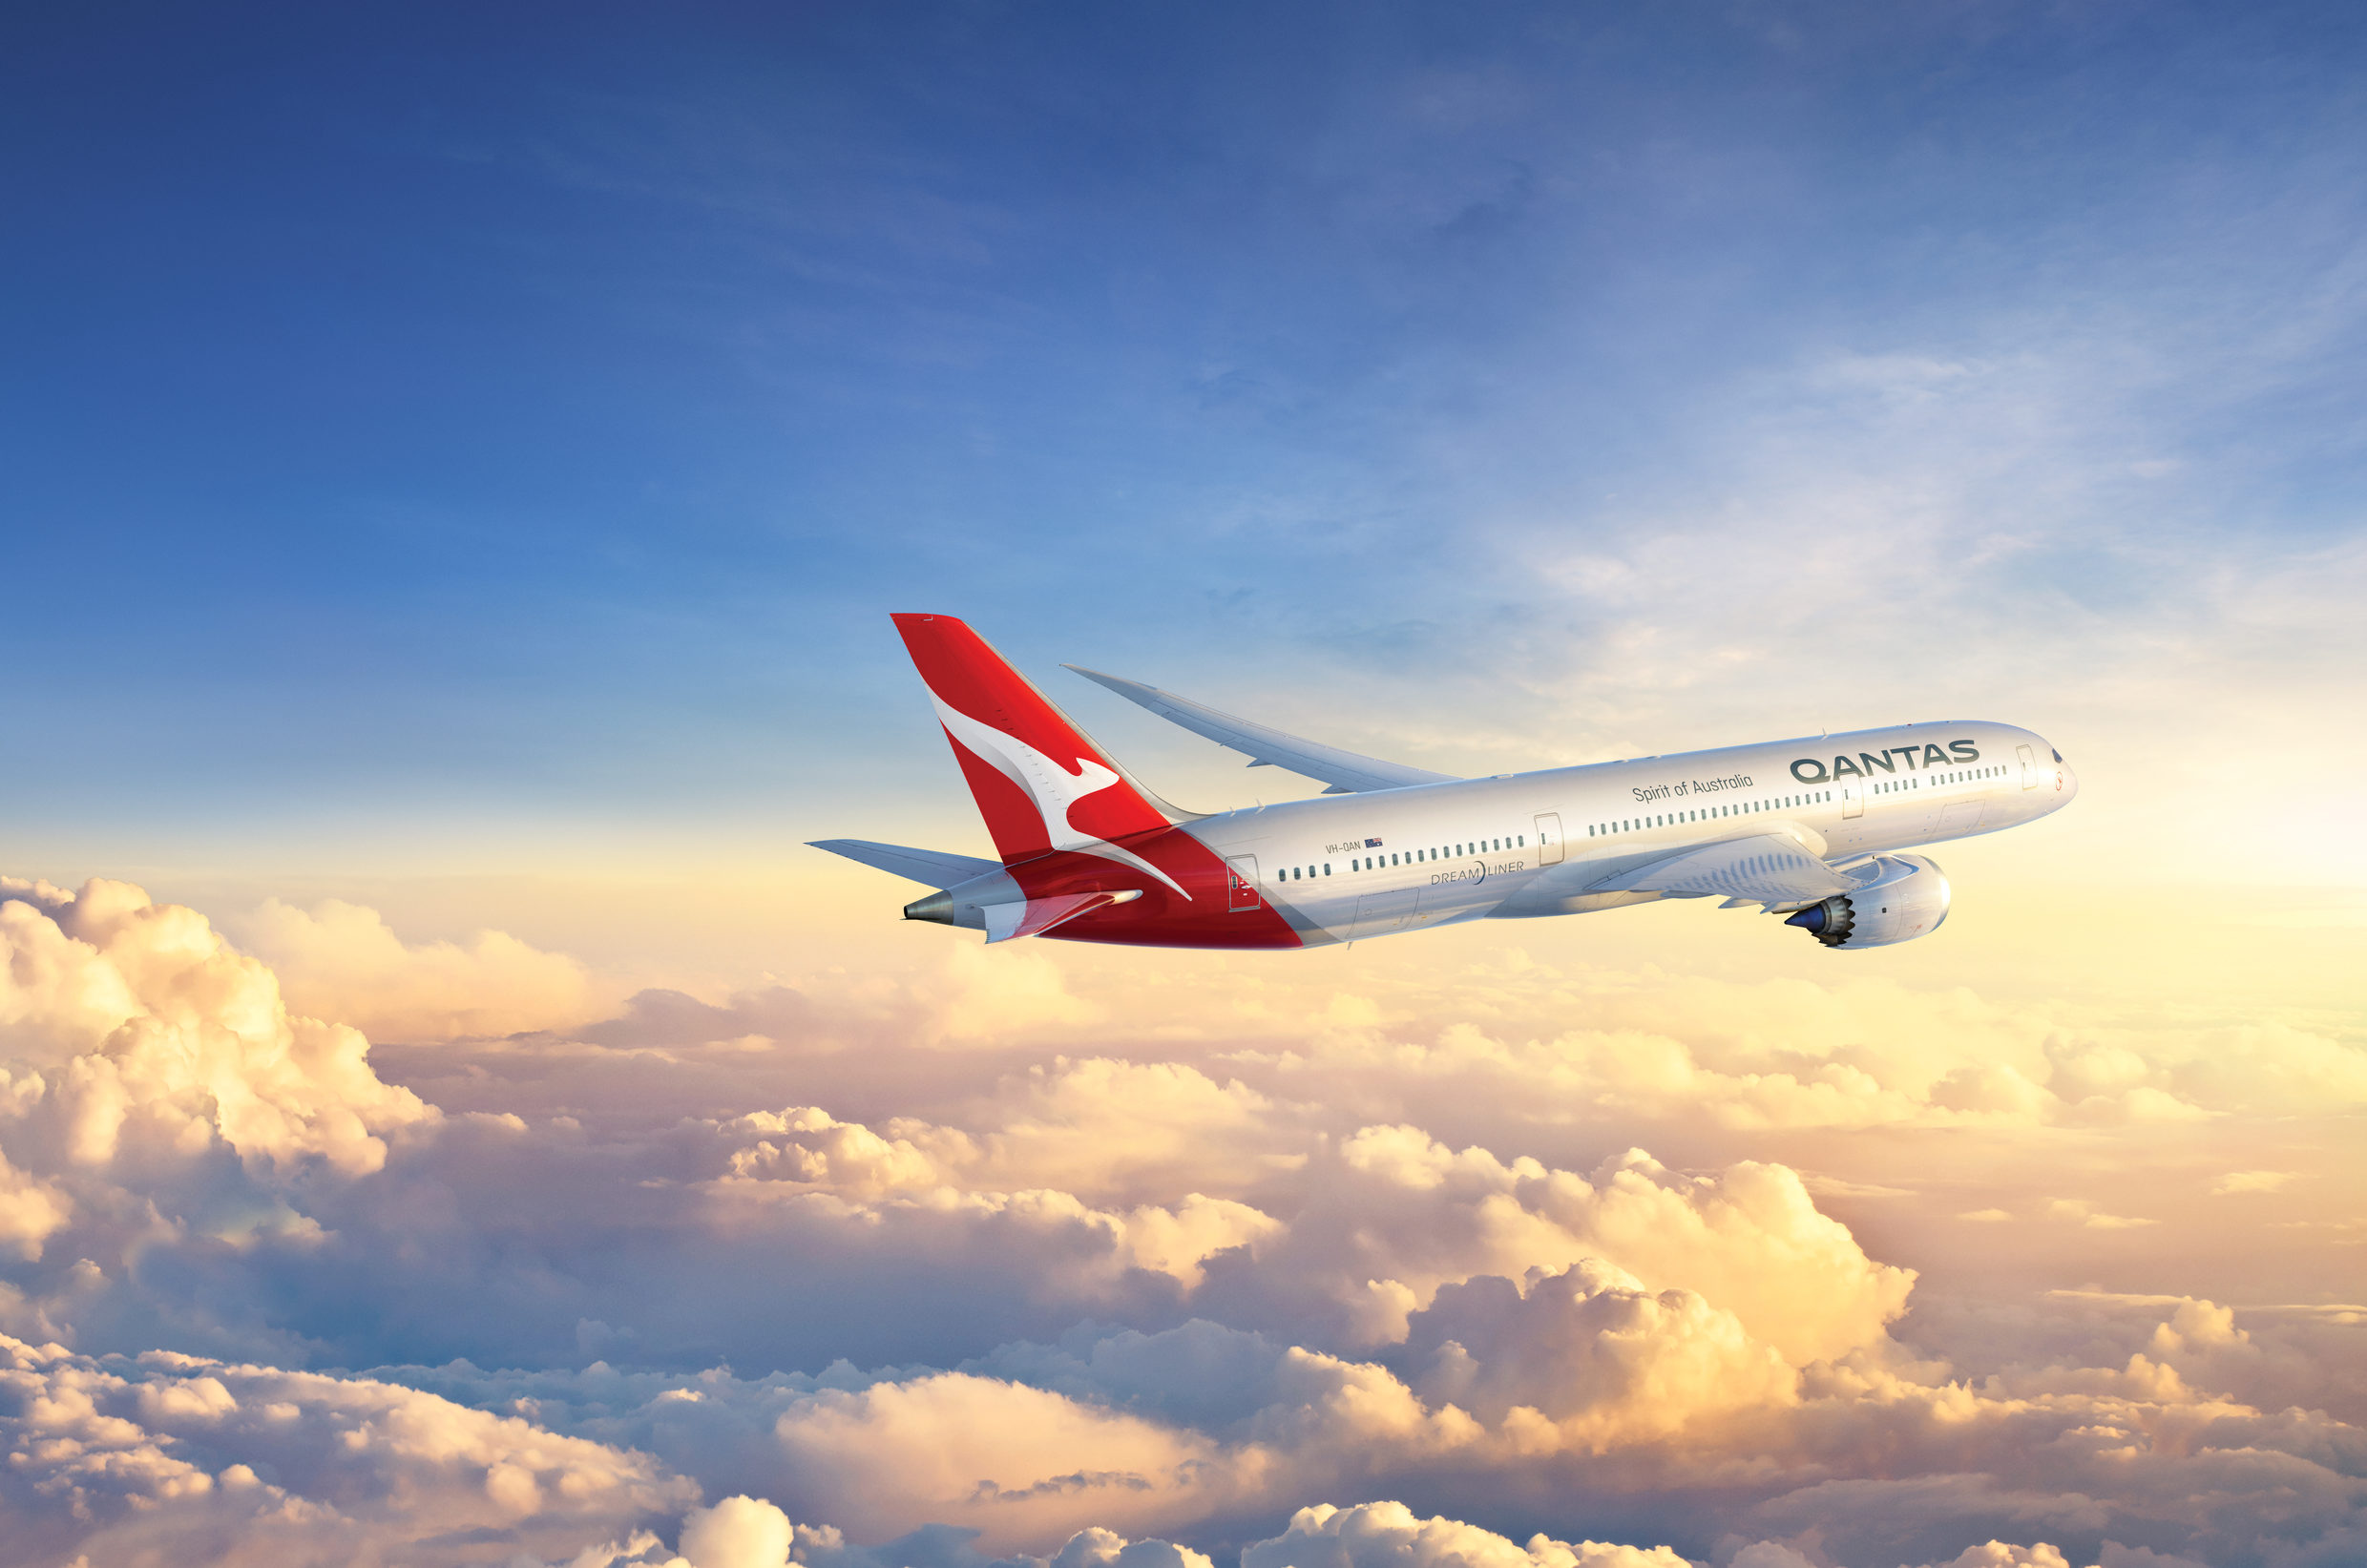
\includegraphics[width=1\textwidth,height=\textheight]{source/figures/full_caption_example.jpg}
\caption{This is not a boat}\label{fig:other_fig}
}
\end{figure}

\hypertarget{research-containing-a-table}{%
\chapter{Research containing a
table}\label{research-containing-a-table}}

\hypertarget{introduction-3}{%
\section{Introduction}\label{introduction-3}}

This is the introduction. Phasellus non purus id mauris aliquam rutrum
vitae quis tellus. Maecenas rhoncus ligula nulla, fringilla placerat mi
consectetur eu. Aenean nec metus ac est ornare posuere. Nunc ipsum
lacus, gravida commodo turpis quis, rutrum eleifend erat. Pellentesque
id lorem eget ante porta tincidunt nec nec tellus.

\hypertarget{method-2}{%
\section{Method}\label{method-2}}

Vivamus consectetur, velit in congue lobortis, massa massa lacinia urna,
sollicitudin semper ipsum augue quis tortor. Donec quis nisl at arcu
volutpat ultrices. Maecenas ex nibh, consequat ac blandit sit amet,
molestie in odio. Morbi finibus libero et nisl dignissim, at ultricies
ligula pulvinar.

\hypertarget{subsection-1-1}{%
\subsection{Subsection 1}\label{subsection-1-1}}

This is the first part of the methodology. Integer leo erat, commodo in
lacus vel, egestas varius elit. Nulla eget magna quam. Nullam
sollicitudin dolor ut ipsum varius tincidunt. Duis dignissim massa in
ipsum accumsan imperdiet. Maecenas suscipit sapien sed dui pharetra
blandit. Morbi fermentum est vel quam pretium maximus.

\hypertarget{subsection-2-2}{%
\subsection{Subsection 2}\label{subsection-2-2}}

This is the second part of the methodology. Nullam accumsan condimentum
eros eu volutpat. Maecenas quis ligula tempor, interdum ante sit amet,
aliquet sem. Fusce tellus massa, blandit id tempus at, cursus in tortor.
Nunc nec volutpat ante. Phasellus dignissim ut lectus quis porta. Lorem
ipsum dolor sit amet, consectetur adipiscing elit.

\hypertarget{results-2}{%
\section{Results}\label{results-2}}

Table \ref{tbl:random} shows us how to add a table. Integer tincidunt
sed nisl eget pellentesque. Mauris eleifend, nisl non lobortis
fringilla, sapien eros aliquet orci, vitae pretium massa neque eu
turpis. Pellentesque tincidunt aliquet volutpat. Ut ornare dui id ex
sodales laoreet.

\newpage

\begin{longtable}[]{@{}lcccccc@{}}
\caption{Important data for various land masses.
\label{tbl:random}}\tabularnewline
\toprule
\begin{minipage}[b]{0.12\columnwidth}\raggedright
Landmass\strut
\end{minipage} & \begin{minipage}[b]{0.08\columnwidth}\centering
\% stuff\strut
\end{minipage} & \begin{minipage}[b]{0.10\columnwidth}\centering
Number of Owls\strut
\end{minipage} & \begin{minipage}[b]{0.14\columnwidth}\centering
Dolphins per Capita\strut
\end{minipage} & \begin{minipage}[b]{0.12\columnwidth}\centering
How Many Foos\strut
\end{minipage} & \begin{minipage}[b]{0.12\columnwidth}\centering
How Many Bars\strut
\end{minipage} & \begin{minipage}[b]{0.12\columnwidth}\centering
Forbidden Float\strut
\end{minipage}\tabularnewline
\midrule
\endfirsthead
\toprule
\begin{minipage}[b]{0.12\columnwidth}\raggedright
Landmass\strut
\end{minipage} & \begin{minipage}[b]{0.08\columnwidth}\centering
\% stuff\strut
\end{minipage} & \begin{minipage}[b]{0.10\columnwidth}\centering
Number of Owls\strut
\end{minipage} & \begin{minipage}[b]{0.14\columnwidth}\centering
Dolphins per Capita\strut
\end{minipage} & \begin{minipage}[b]{0.12\columnwidth}\centering
How Many Foos\strut
\end{minipage} & \begin{minipage}[b]{0.12\columnwidth}\centering
How Many Bars\strut
\end{minipage} & \begin{minipage}[b]{0.12\columnwidth}\centering
Forbidden Float\strut
\end{minipage}\tabularnewline
\midrule
\endhead
\begin{minipage}[t]{0.12\columnwidth}\raggedright
North America\strut
\end{minipage} & \begin{minipage}[t]{0.08\columnwidth}\centering
94\%\strut
\end{minipage} & \begin{minipage}[t]{0.10\columnwidth}\centering
20,028\strut
\end{minipage} & \begin{minipage}[t]{0.14\columnwidth}\centering
17,465\strut
\end{minipage} & \begin{minipage}[t]{0.12\columnwidth}\centering
12,084\strut
\end{minipage} & \begin{minipage}[t]{0.12\columnwidth}\centering
20,659\strut
\end{minipage} & \begin{minipage}[t]{0.12\columnwidth}\centering
1.71\strut
\end{minipage}\tabularnewline
\begin{minipage}[t]{0.12\columnwidth}\raggedright
Central America\strut
\end{minipage} & \begin{minipage}[t]{0.08\columnwidth}\centering
91\%\strut
\end{minipage} & \begin{minipage}[t]{0.10\columnwidth}\centering
6564\strut
\end{minipage} & \begin{minipage}[t]{0.14\columnwidth}\centering
6350\strut
\end{minipage} & \begin{minipage}[t]{0.12\columnwidth}\centering
8,189\strut
\end{minipage} & \begin{minipage}[t]{0.12\columnwidth}\centering
12,012\strut
\end{minipage} & \begin{minipage}[t]{0.12\columnwidth}\centering
1.52\strut
\end{minipage}\tabularnewline
\begin{minipage}[t]{0.12\columnwidth}\raggedright
South America\strut
\end{minipage} & \begin{minipage}[t]{0.08\columnwidth}\centering
86\%\strut
\end{minipage} & \begin{minipage}[t]{0.10\columnwidth}\centering
3902\strut
\end{minipage} & \begin{minipage}[t]{0.14\columnwidth}\centering
4127\strut
\end{minipage} & \begin{minipage}[t]{0.12\columnwidth}\centering
5,205\strut
\end{minipage} & \begin{minipage}[t]{0.12\columnwidth}\centering
6,565\strut
\end{minipage} & \begin{minipage}[t]{0.12\columnwidth}\centering
1.28\strut
\end{minipage}\tabularnewline
\begin{minipage}[t]{0.12\columnwidth}\raggedright
Africa\strut
\end{minipage} & \begin{minipage}[t]{0.08\columnwidth}\centering
84\%\strut
\end{minipage} & \begin{minipage}[t]{0.10\columnwidth}\centering
2892\strut
\end{minipage} & \begin{minipage}[t]{0.14\columnwidth}\centering
3175\strut
\end{minipage} & \begin{minipage}[t]{0.12\columnwidth}\centering
3,862\strut
\end{minipage} & \begin{minipage}[t]{0.12\columnwidth}\centering
4,248\strut
\end{minipage} & \begin{minipage}[t]{0.12\columnwidth}\centering
1.1\strut
\end{minipage}\tabularnewline
\begin{minipage}[t]{0.12\columnwidth}\raggedright
Europe\strut
\end{minipage} & \begin{minipage}[t]{0.08\columnwidth}\centering
92\%\strut
\end{minipage} & \begin{minipage}[t]{0.10\columnwidth}\centering
20,964\strut
\end{minipage} & \begin{minipage}[t]{0.14\columnwidth}\centering
17,465\strut
\end{minipage} & \begin{minipage}[t]{0.12\columnwidth}\centering
15,303\strut
\end{minipage} & \begin{minipage}[t]{0.12\columnwidth}\centering
24,203\strut
\end{minipage} & \begin{minipage}[t]{0.12\columnwidth}\centering
1.58\strut
\end{minipage}\tabularnewline
\begin{minipage}[t]{0.12\columnwidth}\raggedright
Asia\strut
\end{minipage} & \begin{minipage}[t]{0.08\columnwidth}\centering
87\%\strut
\end{minipage} & \begin{minipage}[t]{0.10\columnwidth}\centering
6852\strut
\end{minipage} & \begin{minipage}[t]{0.14\columnwidth}\centering
6350\strut
\end{minipage} & \begin{minipage}[t]{0.12\columnwidth}\centering
8,255\strut
\end{minipage} & \begin{minipage}[t]{0.12\columnwidth}\centering
11,688\strut
\end{minipage} & \begin{minipage}[t]{0.12\columnwidth}\centering
1.47\strut
\end{minipage}\tabularnewline
\begin{minipage}[t]{0.12\columnwidth}\raggedright
Oceania\strut
\end{minipage} & \begin{minipage}[t]{0.08\columnwidth}\centering
87\%\strut
\end{minipage} & \begin{minipage}[t]{0.10\columnwidth}\centering
4044\strut
\end{minipage} & \begin{minipage}[t]{0.14\columnwidth}\centering
4127\strut
\end{minipage} & \begin{minipage}[t]{0.12\columnwidth}\centering
5,540\strut
\end{minipage} & \begin{minipage}[t]{0.12\columnwidth}\centering
6,972\strut
\end{minipage} & \begin{minipage}[t]{0.12\columnwidth}\centering
1.28\strut
\end{minipage}\tabularnewline
\begin{minipage}[t]{0.12\columnwidth}\raggedright
Antarctica\strut
\end{minipage} & \begin{minipage}[t]{0.08\columnwidth}\centering
83\%\strut
\end{minipage} & \begin{minipage}[t]{0.10\columnwidth}\centering
2964\strut
\end{minipage} & \begin{minipage}[t]{0.14\columnwidth}\centering
3175\strut
\end{minipage} & \begin{minipage}[t]{0.12\columnwidth}\centering
4,402\strut
\end{minipage} & \begin{minipage}[t]{0.12\columnwidth}\centering
4,941\strut
\end{minipage} & \begin{minipage}[t]{0.12\columnwidth}\centering
1.13\strut
\end{minipage}\tabularnewline
\bottomrule
\end{longtable}

\hypertarget{discussion-2}{%
\section{Discussion}\label{discussion-2}}

This is the discussion. As we saw in Table \ref{tbl:random}, many things
are true, and other things are not. Etiam sit amet mi eros. Donec vel
nisi sed purus gravida fermentum at quis odio. Vestibulum quis nisl sit
amet justo maximus molestie. Maecenas vitae arcu erat. Nulla facilisi.
Nam pretium mauris eu enim porttitor, a mattis velit dictum. Nulla sit
amet ligula non mauris volutpat fermentum quis vitae sapien.

\hypertarget{conclusion-3}{%
\section{Conclusion}\label{conclusion-3}}

This is the conclusion to the chapter. Nullam porta tortor id vehicula
interdum. Quisque pharetra, neque ut accumsan suscipit, orci orci
commodo tortor, ac finibus est turpis eget justo. Cras sodales nibh nec
mauris laoreet iaculis. Morbi volutpat orci felis, id condimentum nulla
suscipit eu. Fusce in turpis quis ligula tempus scelerisque eget quis
odio. Vestibulum et dolor id erat lobortis ullamcorper quis at sem.

\hypertarget{final-research-study}{%
\chapter{Final research study}\label{final-research-study}}

\hypertarget{introduction-4}{%
\section{Introduction}\label{introduction-4}}

This is the introduction. Nunc lorem odio, laoreet eu turpis at,
condimentum sagittis diam. Phasellus metus ligula, auctor ac nunc vel,
molestie mattis libero. Praesent id posuere ex, vel efficitur nibh.
Quisque vestibulum accumsan lacus vitae mattis.

\hypertarget{method-3}{%
\section{Method}\label{method-3}}

In tincidunt viverra dolor, ac pharetra tellus faucibus eget.
Pellentesque tempor a enim nec venenatis. Morbi blandit magna imperdiet
posuere auctor. Maecenas in maximus est.

\hypertarget{subsection-1-2}{%
\subsection{Subsection 1}\label{subsection-1-2}}

This is the first part of the methodology. Praesent mollis sem diam, sit
amet tristique lacus vulputate quis. Vivamus rhoncus est rhoncus tellus
lacinia, a interdum sem egestas. Curabitur quis urna vel quam blandit
semper vitae a leo. Nam vel lectus lectus.

\hypertarget{subsection-2-3}{%
\subsection{Subsection 2}\label{subsection-2-3}}

This is the second part of the methodology. Aenean vel pretium tortor.
Aliquam erat volutpat. Quisque quis lobortis mi. Nulla turpis leo,
ultrices nec nulla non, ullamcorper laoreet risus.

\hypertarget{results-3}{%
\section{Results}\label{results-3}}

These are the results. Curabitur vulputate nisl non ante tincidunt
tempor. Aenean porta nisi quam, sed ornare urna congue sed. Curabitur in
sapien justo. Quisque pulvinar ullamcorper metus, eu varius mauris
pellentesque et. In hac habitasse platea dictumst. Pellentesque nec
porttitor libero. Duis et magna a massa lacinia cursus.

\hypertarget{discussion-3}{%
\section{Discussion}\label{discussion-3}}

This is the discussion. Curabitur gravida nisl id gravida congue. Duis
est nisi, sagittis eget accumsan ullamcorper, semper quis turpis. Mauris
ultricies diam metus, sollicitudin ultricies turpis lobortis vitae. Ut
egestas vehicula enim, porta molestie neque consectetur placerat.
Integer iaculis sapien dolor, non porta nibh condimentum ut.

\hypertarget{conclusion-4}{%
\section{Conclusion}\label{conclusion-4}}

This is the conclusion to the chapter. Nulla sed condimentum lectus.
Duis sed tempor erat, at cursus lacus. Nam vitae tempus arcu, id
vestibulum sapien. Cum sociis natoque penatibus et magnis dis parturient
montes, nascetur ridiculus mus.

\hypertarget{conclusion-5}{%
\chapter{Conclusion}\label{conclusion-5}}

\hypertarget{thesis-summary}{%
\section{Thesis summary}\label{thesis-summary}}

In summary, pellentesque habitant morbi tristique senectus et netus et
malesuada fames ac turpis egestas. Nunc eleifend, ex a luctus porttitor,
felis ex suscipit tellus, ut sollicitudin sapien purus in libero. Nulla
blandit eget urna vel tempus. Praesent fringilla dui sapien, sit amet
egestas leo sollicitudin at.

\hypertarget{future-work}{%
\section{Future work}\label{future-work}}

There are several potential directions for extending this thesis. Lorem
ipsum dolor sit amet, consectetur adipiscing elit. Aliquam gravida ipsum
at tempor tincidunt. Aliquam ligula nisl, blandit et dui eu, eleifend
tempus nibh. Nullam eleifend sapien eget ante hendrerit commodo.
Pellentesque pharetra erat sit amet dapibus scelerisque.

Vestibulum suscipit tellus risus, faucibus vulputate orci lobortis eget.
Nunc varius sem nisi. Nunc tempor magna sapien, euismod blandit elit
pharetra sed. In dapibus magna convallis lectus sodales, a consequat sem
euismod. Curabitur in interdum purus. Integer ultrices laoreet aliquet.
Nulla vel dapibus urna. Nunc efficitur erat ac nisi auctor sodales.

\hypertarget{appendix-1-some-extra-stuff}{%
\chapter*{Appendix 1: Some extra
stuff}\label{appendix-1-some-extra-stuff}}
\addcontentsline{toc}{chapter}{Appendix 1: Some extra stuff}

Add appendix 1 here. Vivamus hendrerit rhoncus interdum. Sed ullamcorper
et augue at porta. Suspendisse facilisis imperdiet urna, eu pellentesque
purus suscipit in. Integer dignissim mattis ex aliquam blandit.
Curabitur lobortis quam varius turpis ultrices egestas.

\hypertarget{appendix-2-some-more-extra-stuff}{%
\chapter*{Appendix 2: Some more extra
stuff}\label{appendix-2-some-more-extra-stuff}}
\addcontentsline{toc}{chapter}{Appendix 2: Some more extra stuff}

Add appendix 2 here. Aliquam rhoncus mauris ac neque imperdiet, in
mattis eros aliquam. Etiam sed massa et risus posuere rutrum vel et
mauris. Integer id mauris sed arcu venenatis finibus. Etiam nec
hendrerit purus, sed cursus nunc. Pellentesque ac luctus magna. Aenean
non posuere enim, nec hendrerit lacus. Etiam lacinia facilisis tempor.
Aenean dictum nunc id felis rhoncus aliquam.

\footnotesize
\singlespacing
\setlength{\parindent}{0in}

\hypertarget{references}{%
\chapter*{References}\label{references}}
\addcontentsline{toc}{chapter}{References}

\hypertarget{refs}{}
\begin{CSLReferences}{1}{0}
\leavevmode\hypertarget{ref-Cousteau1963}{}%
Cousteau Jacques \& Dugan James, 1963. \emph{{The Living Sea: by
Jacques-Yves Cousteau}}, London: Hamish Hamilton.

\end{CSLReferences}

\end{document}
